\documentclass{article}
\usepackage{graphicx} % Required for inserting images
\usepackage{amsmath}
\usepackage{amsfonts}
\usepackage[margin=2.5cm]{geometry}


\title{CS229 - Problem Set 1}
\author{Or Haifler}
\date{November 2023}

\begin{document}

\maketitle

\section*{Exercise 1}
\subsection*{(a)}
\begin{align*}
    & J(\theta)=-\frac{1}{m}\Bigg{[}\sum_{i=1}^{m}y^{(i)}\log(h_{\theta}(x^{(i)}))+(1-y^{(i)})\log(1-h_{\theta}(x^{(i)}))\Bigg{]}                                                                                                                                                                                                                        \\
    & \frac{\partial}{\partial\theta_{k}\theta_{j}}\log(h_{\theta}(x))=-x_{k}x_{j}h_{\theta}(x)(1-h_{\theta}(x)), \frac{\partial}{\partial\theta_{k}\theta_{j}}\log(1-h_{\theta}(x))=-x_{k}x_{j}h_{\theta}(x)(1-h_{\theta}(x))                                                                                                                           \\
    & \frac{\partial}{\partial\theta_{k}\theta_{j}}J(\theta)=-\frac{1}{m}\Bigg{[}\sum_{i=1}^{m}y^{(i)}\frac{\partial}{\partial\theta_{k}\theta_{j}}\log(h_{\theta}(x^{(i)}))+(1-y^{(i)})\frac{\partial}{\partial\theta_{k}\theta_{j}}\log(1-h_{\theta}(x^{(i)}))\Bigg{]} = \frac{1}{m}\sum_{i=1}^{m}x_{j}x_{k}h_{\theta}(x^{(i)})(1-h_{\theta}(x^{(i)})) \\
    & \langle Hz,z \rangle = \sum_{k=1}^{n}\sum_{j=1}^{n}z_{j}z_{k}\frac{1}{m}\sum_{i=1}^{m}x_{j}x_{k}h_{\theta}(x^{(i)})(1-h_{\theta}(x^{(i)}))=\frac{1}{m}\Bigg{(}\sum_{i=1}^{m}h_{\theta}(x^{(i)})(1-h_{\theta}(x^{(i)}))\Bigg{)}\sum_{k=1}^{n}\sum_{j=1}^{n}z_{j}z_{k}x_{j}x_{k} = \frac{\lambda}{m}(x^{T}z)^2 \ge 0
\end{align*}


\subsubsection*{(c)}

\begin{align*}
    & p(y=1|x;\phi,\mu_{0},\mu_{1},\Sigma) = \frac{p(x|y=1)p(y=1)}{p(x|y=0)p(y=0)+p(x|y=1)p(y=1)}                                                                                                                                                                                                                        \\
    & =\frac{\frac{\phi}{(2\pi)^{n/2}\det(\Sigma)^{1/2}}\exp(-\frac{1}{2}(x-\mu_{1})^{T}\Sigma^{-1}(x-\mu_{1})}{\frac{1-\phi}{(2\pi)^{n/2}\det(\Sigma)^{1/2}}\exp(-\frac{1}{2}(x-\mu_{0})^{T}\Sigma^{-1}(x-\mu_{0})) +\frac{\phi}{(2\pi)^{n/2}\det(\Sigma)^{1/2}}\exp(-\frac{1}{2}(x-\mu_{1})^{T}\Sigma^{-1}(x-\mu_{1})} \\
    & = \frac{\exp(-\frac{1}{2}(x-\mu_{1})^{T}\Sigma^{-1}(x-\mu_{1}))}{\frac{1-\phi}{\phi}\exp(-\frac{1}{2}(x-\mu_{0})^{T}\Sigma^{-1}(x-\mu_{0}))+\exp(-\frac{1}{2}(x-\mu_{1})^{T}\Sigma^{-1}(x-\mu_{1}))}                                                                                                               \\
    & = \frac{1}{1 + \frac{1-\phi}{\phi}\exp(-\frac{1}{2}((x-\mu_{0})^{T}\Sigma^{-1}(x-\mu_{0})-(x-\mu_{1})^{T}\Sigma^{-1}(x-\mu_{1}))}                                                                                                                                                                                  \\
    & = \frac{1}{1+\exp(-\frac{1}{2}(\mu_{1}-\mu_{0})^T\Sigma^{-1}x+\frac{1}{2}(\mu_{1}^{T}\Sigma^{-1}\mu_{1}-\mu_{0}^{T}\Sigma^{-1}\mu_{0})+\log(\frac{1-\phi}{\phi}))}=\frac{1}{1+\exp(-(\theta^{T}x+\theta_{0}))}                                                                                                     \\
    & \theta=(\Sigma^T)^{-1}(\mu_{1}-\mu_{0})\overset{\Sigma^{T}=\Sigma}{=}\Sigma^{-1}(\mu_{1}-\mu_{0}),\theta_{0}=\frac{1}{2}(\mu_{1}^{T}\Sigma^{-1}\mu_{1}-\mu_{0}^{T}\Sigma^{-1}\mu_{0})+\log(\frac{1-\phi}{\phi})
\end{align*}

\subsection*{(d)}

\begin{align*}
    & \frac{\partial}{\partial\phi}\ell(\phi,\mu_{0},\mu_{1},\sigma)=\frac{\partial}{\partial\phi}\log\prod_{i=1}^{m}p(x^{(i)}|y^{(i)};\mu_{0},\mu_{1},\Sigma)p(y^{(i)};\phi)=\sum_{i=1}^{m}\frac{\partial}{\partial\phi}\log p(x^{(i)}|y^{(i)};\mu_{0},\mu_{1},\sigma)p(y^{(i)};\phi)                       \\
    & \sum_{i=1}^{m}\frac{\partial}{\partial\phi}\log p(y^{(i)};\phi)=\sum_{i=1}^{m_{0}}\frac{\partial}{\partial\phi}\log\phi+\sum_{i=m_{0}}^{m}\frac{\partial}{\partial\phi}\log(1-\phi)=\frac{m_{0}}{\phi}+\frac{m-m_{0}}{1-\phi}                                                                          \\
    & \frac{\partial}{\partial\phi}\ell(\phi,\mu_{0},\mu_{1},\sigma)= 0 \implies (1-\phi)m_{0}+\phi(m_{0}-m)=0 \implies \phi = \frac{m_0}{m} = \frac{1}{m}\sum_{i=1}^{m}\mathbbm{1}\{y^{(i)}=1\}                                                                                                             \\
    & \nabla_{\mu_{0}}\ell(\phi,\mu_{0},\mu_{1},\sigma)=\sum_{i=1}^{m}\nabla_{\mu_{0}}\log p(x^{(i)}|y^{(i)};\mu_{0},\mu_{1},\sigma)                                                                                                                                                                         \\
    & =\sum_{i=m_{0}}^{m}\nabla_{\mu_{0}}\log\frac{1}{(2\pi)^{n/2}\det(\sigma)^{1/2}}\exp(-\frac{1}{2}(x^{(i)}-\mu_{0})^{T}\sigma^{-1}(x^{(i)}-\mu_{0})) =                                                                                                                                                   \\
    & = -\frac{1}{2}\sum_{i=m_{0}}^{m}\nabla_{\mu_{0}}(x^{(i)}-\mu_{0})^{T}\sigma^{-1}(x^{(i)}-\mu_{0})
  = \sum_{i=m_{0}}^{m}\sigma^{-1}(x^{(i)}-\mu_{0}) \\
    & \nabla_{\mu_{0}}\ell(\phi,\mu_{0},\mu_{1},\sigma)=0 \implies \sum_{i=m_{0}}^{m}(x^{(i)}-\mu_{0})=0\implies \mu_{0}=\frac{\sum_{i=m_0}^{m}\mathbbm{1}\{{y^{(i)}=0}\}x^{(i)}}{\sum_{i=m_0}^{m}\mathbbm{1}\{{y^{(i)}=0}\}}                                                                                \\
    & \nabla_{\mu_{1}}\ell(\phi,\mu_{0},\mu_{1},\sigma)=0 \implies \sum_{i=0}^{m_{0}}(x^{(i)}-\mu_{1})=0\implies \mu_{1}=\frac{\sum_{i=0}^{m_{0}}\mathbbm{1}\{{y^{(i)}=1}\}x^{(i)}}{\sum_{i=0}^{m_{0}}\mathbbm{1}\{{y^{(i)}=1}\}}                                                                            \\
    & \frac{\partial}{\partial\sigma}\ell(\phi,\mu_{0},\mu_{1},\sigma)=\sum_{i=1}^{m}\frac{\partial}{\partial\sigma}\log p(x^{(i)}|y^{(i)};\mu_{0},\mu_{1},\sigma)=-\frac{m}{2\sigma}-\frac{1}{2}\frac{\partial}{\partial\sigma}\sigma^{-1}\sum_{i=1}^{m}(x^{(i)}-\mu_{y^{(i)}})^{T}(x^{(i)}-\mu_{y^{(i)}})= \\
    & -\frac{m}{2\sigma}+\frac{1}{2\sigma^{2}}\sum_{i=1}^{m}(x^{(i)}-\mu_{y^{(i)}})^{T}(x^{(i)}-\mu_{y^{(i)}})                                                                                                                                                                                               \\
    & \frac{\partial}{\partial\sigma}\ell(\phi,\mu_{0},\mu_{1},\sigma)=0\implies m=\frac{1}{\sigma}\sum_{i=1}^{m}(x^{(i)}-\mu_{y^{(i)}})^{T}(x^{(i)}-\mu_{y^{(i)}})\implies\sigma=\frac{1}{m}\sum_{i=1}^{m}(x^{(i)}-\mu_{y^{(i)}})^{T}(x^{(i)}-\mu_{y^{(i)}})
\end{align*}

\newpage

\subsection*{(g)}

\begin{figure}[h]
  \centering
  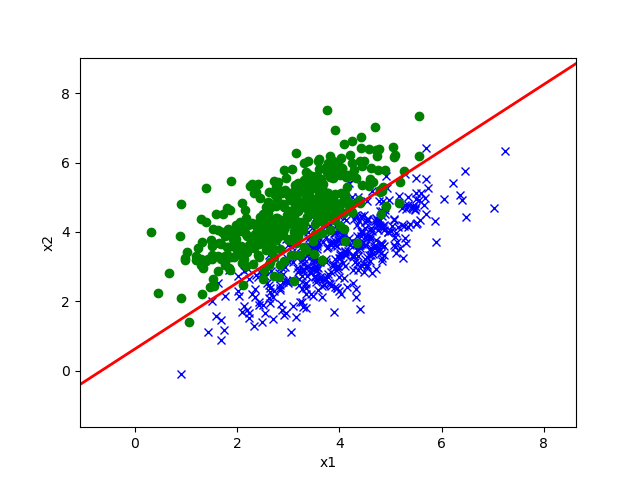
\includegraphics[width=1\textwidth]{images/p01b.png}
  \caption{GDA}
  \label{fig:enter-label}
\end{figure}

\begin{figure}
  \centering
  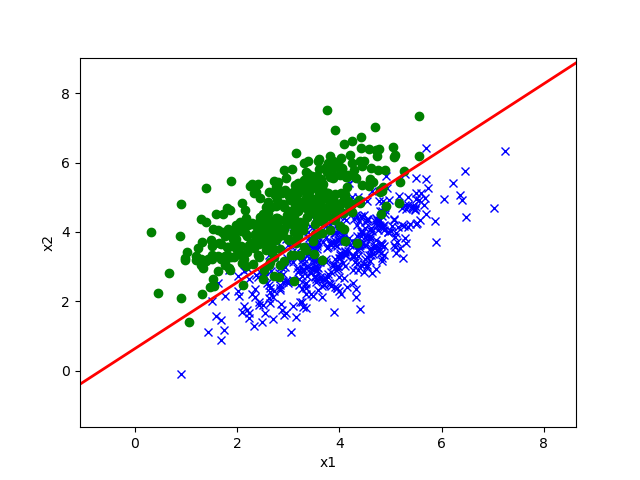
\includegraphics[width=1\textwidth]{images/01e.png}
  \caption{Logistic Regression}
  \label{fig:enter-label}
\end{figure}

\section*{Exercise 2}
\subsection*{(a)}

\begin{align*}
    & p(y=1|t=1,x)p(t=1|x)p(x)=p(y=1,t=1,x)=p(t=1|y=1,x)p(y=1|x)p(x) \\
    & p(t=1|x)=p(y=1|x)\frac{p(t=1|y=1,x)}{p(y=1|t=1,x}              \\
    & p(t=1|y=1,x)=1,p(y=1|t=1,x)=p(y=1|t=1)                         \\
    & p(t=1|x)=\frac{p(y=1|x)}{p(y=1|t=1)},p(y=1|t=1)=\alpha
\end{align*}

\subsection*{(b)}

\begin{align*}
  h(x^{(i)})\approx(y^{(i)}=1|x^{(i)})\overset{(a)}{=}\alpha p(t^{(i)}=1|x^(i))\approx \alpha
\end{align*}

\newpage

\subsection*{(c)}

\begin{figure}[h]
  \centering
  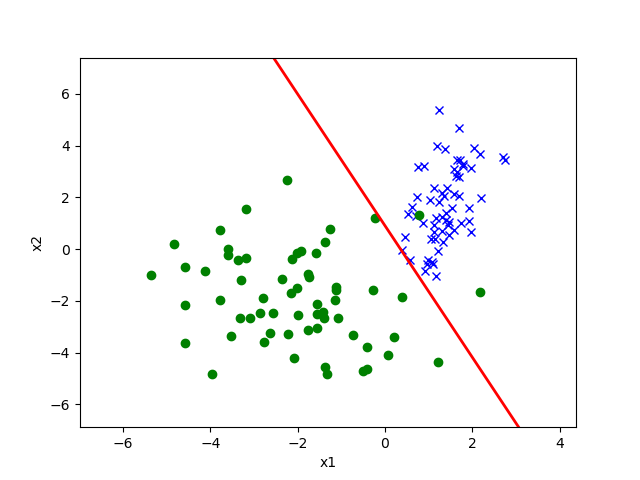
\includegraphics[width=1\textwidth]{images/p02c_test.png}
  \caption{t-labels}
  \label{fig:enter-label}
\end{figure}

\newpage

\subsection*{(d)}

\begin{figure}[h]
  \centering
  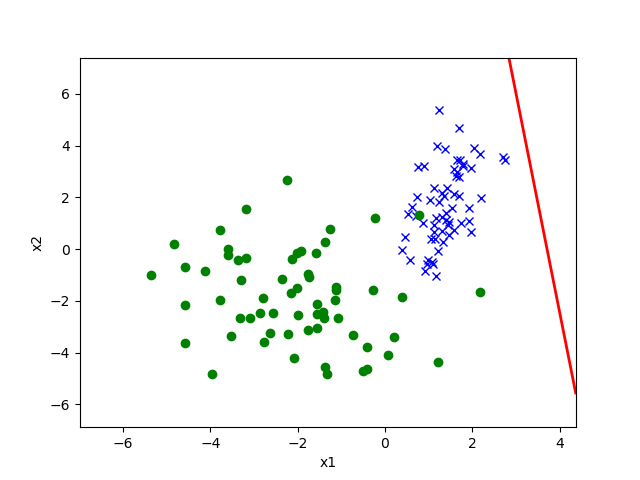
\includegraphics[width=1\textwidth]{images/p02d_test.png}
  \caption{y-labels}
  \label{fig:enter-label}
\end{figure}

\newpage

\section*{Exercise 3}
\subsection*{(a)}

\begin{align*}
    & p(y;\lambda)=\frac{1}{y!}\exp(y\ln(\lambda)-\lambda)=b(y)\exp(T(y)\eta-a(\eta)) \\
    & b(y)=\frac{1}{y!},T(y)=y,\eta=\ln(\lambda),a(\eta)=\exp(\eta)
\end{align*}

\subsection*{(b)}

\begin{align*}
    & g(\eta)=\mathbb{E}[T(y);\eta]=\mathbb{E}[y;\eta],y\sim\text{Poisson}(\lambda)\implies g(\eta)=\lambda=\exp(\eta)
\end{align*}

\subsection*{(c)}

\begin{align*}
    & p(y^{(i)}|x^{(i)};\theta)=\frac{1}{y!}\exp(y^{(i)}\theta^{T}x^{(i)}-\exp(\theta^{T}x^{(i)}))                                                                          \\
    & \frac{\partial}{\partial\theta_{j}}\log p(y^{(i)}|x^{(i)};\theta)=\frac{\partial}{\partial\theta_{j}}\Bigg{(}y^{(i)}\theta^{T}x^{(i)}-\exp(\theta^{T}x^{(i)})\Bigg{)} \\
    & = x^{(i)}_j(y^{(i)}-\exp(\theta^{T}x^{(i)})), \theta_{j} := \theta_{j} + \alpha x^{(i)}_j(y^{(i)}-\exp(\theta^{T}x^{(i)}))
\end{align*}

\newpage

\subsection*{(d)}

\begin{figure}[h]
  \centering
  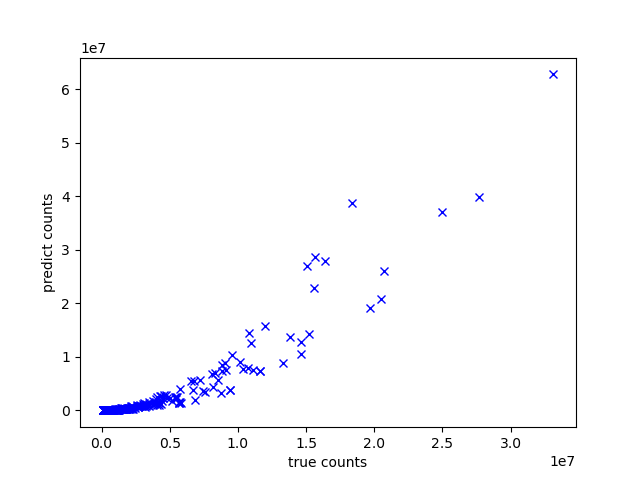
\includegraphics[width=1\textwidth]{images/p03d.png}
\end{figure}

\newpage

\section*{Exercise 4}
\subsection*{(a)}
\begin{align*}
    & \mathbb{E}[y|x;\theta]=\mathbb{E}[b(y)\exp(\eta y-a(\eta))]=\int_{-\infty}^{\infty}yb(y)\exp(\eta y-a(\eta))                                                                                                                        \\
    & \frac{\partial a(\eta)}{\partial\eta}\int_{-\infty}^{\infty}p(y;\eta)=\int_{-\infty}^{\infty}\frac{\partial a(\eta)}{\partial\eta}p(y;\eta)=\int_{-\infty}^{\infty}b(y)(y-\frac{\partial a(\eta)}{\partial\eta}\exp(\eta y-a(\eta)) \\
    & =\int_{-\infty}^{\infty}yb(y)\exp(\eta y-a(\eta))-\frac{\partial a(\eta)}{\partial\eta}\int_{-\infty}^{\infty}b(y)\exp(\eta y-a(\eta))=\mathbb{E}[y|x;\theta]-\frac{\partial a(\eta)}{\partial\eta}                                 \\
    & \mathbb{E}[y|x;\theta]-\frac{\partial a(\eta)}{\partial\eta}=\frac{\partial a(\eta)}{\partial\eta}\int_{-\infty}^{\infty}p(y;\eta)=0\implies \mathbb{E}[y|x;\theta]=\frac{\partial a(\eta)}{\partial\eta}
\end{align*}

\subsection*{(b)}
\begin{align*}
    & \frac{\partial^{2}a(\eta)}{\partial\eta^{2}}=\frac{\partial}{\partial\eta}\mathbb{E}[y|x;\theta]=\int_{-\infty}^{\infty}\frac{\partial }{\partial\eta}yp(y|x;\theta)=\int_{-\infty}^{\infty}yb(y)(y-\frac{\partial a(\eta)}{\partial\eta}\exp(\eta y-a(\eta)) \\
    & =\int_{-\infty}^{\infty}y^{2}b(y)\exp(\eta y-a(\eta))-\frac{\partial a(\eta)}{\partial\eta}\int_{-\infty}^{\infty}yb(y)\exp(\eta y-a(\eta)) =\mathbb{E}[y^{2}|x;\theta]-\mathbb{E}[y|x;\theta]^{2}=\text{Var}[y|x;\theta]
\end{align*}

\subsection*{(c)}
\begin{align*}
    & \frac{\partial}{\partial\theta_{k}\theta_{j}}\ell(\theta)=-\sum_{i=1}^{m}\frac{\partial}{\partial\theta_{k}\theta_{j}}\log p(y^{(i)}|x^{(i)};\theta)=-\sum_{i=1}^{m}\frac{\partial}{\partial\theta_{k}\theta_{j}}(y^{(i)}\eta-a(\theta^{T}x^{(i)})) \\
    & =\sum_{i=1}^{m}\frac{\partial}{\partial\theta_{k}\theta_{j}}a(\theta^{T}x^{(i)})=\sum_{i=1}^{m}x_{j}^{(i)}x_{k}^{(i)}\frac{\partial^{2}a(\eta)}{\partial\eta^{2}}(\theta^{T}x^{(i)})=\sum_{i=1}^{m}x_{j}^{(i)}x_{k}^{(i)}\text{Var}[Y|X;\theta]     \\
    & \langle Hz,z \rangle = \sum_{i=1}^{m}\sum_{j=1}^{n}\sum_{k=1}^{n}z_{j}z_{k}x_{j}^{(i)}x_{k}^{(i)}\text{Var}[y|x^{(i)};\theta]=\sum_{i=1}^{m}(z^{T}x^{(i)})^{2}\text{Var}[y|x^{(i)};\theta]\ge0
\end{align*}

\newpage

\section{Exercise 5}
\subsection*{(a)}
\subsubsection*{(i).}
\begin{align*}
  W_{ij}=\begin{cases}
    0,                  & \text{if $i\not = j$ odd} \\
    \frac{1}{2}w^{(i)}, & \text{if $i=j$}
  \end{cases}
\end{align*}

\subsubsection*{(ii).}
\begin{align*}
    & \nabla_{\theta}J(\theta)=\nabla_{\theta}(X\theta-y)^{T}W(X\theta-y)=\nabla_{\theta}\Big((X\theta)^{T}WX\theta-(X\theta)^{T}Wy-y^{T}WX\theta+y^{T}Wy)\Big)            \\
    & =\nabla_{\theta}(X\theta)^{T}WX\theta-\nabla_{\theta}(X\theta)^{T}Wy-\nabla_{\theta}y^{T}WX\theta=\nabla_{\theta}(X\theta)^{T}WX\theta-2\nabla_{\theta}y^{T}WX\theta \\
    & =\nabla_{\theta}(X\theta)^{T}WX\theta-2\nabla_{\theta}(X^{T}Wy)^{T}\theta=2X^{T}WX\theta-2X^{T}Wy                                                                    \\
    & \nabla_{\theta}J(\theta)=0\implies X^{T}WX\theta=X^{T}Wy\implies\theta=(X^{T}WX)^{-1}X^{T}Wy
\end{align*}

\subsubsection*{(iii).}
\begin{align*}
    & \ell(\theta)=\log\prod_{i=1}^{m}p(y^{(i)}|x^{(i)};\theta)=\sum_{i=1}^{m}\log\frac{1}{\sqrt{2\pi}\sigma^{(i)}}\exp\Big(-\frac{(y^{(i)}-\theta^{T}x^{(i)})^{2}}{2(\sigma^{(i)})^{2}}\Big)                                                                                          \\
    & =\sum_{i=1}^{m}\log\frac{1}{\sqrt{2\pi}\sigma^{(i)}}-\sum_{i=1}^{m}\frac{(y^{(i)}-\theta^{T}x^{(i)})^{2}}{2(\sigma^{(i)})^{2}},\frac{\partial\ell(\theta)}{\partial\theta_{j}}=\sum_{i=1}^{m}w^{(i)}(y^{(i)}-\theta^{T}x^{(i)})x_{j}^{(i)},w^{(i)}=-\frac{1}{(\sigma^{(i)})^{2}}
\end{align*}

\newpage

\subsection*{(b)}
\begin{figure}[h]
  \centering
  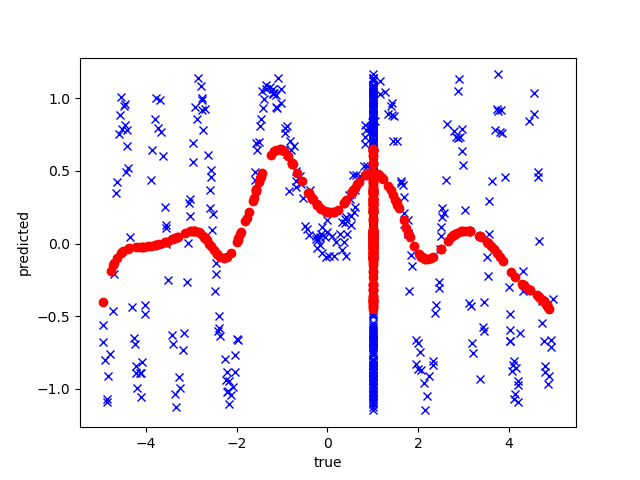
\includegraphics[width=1\textwidth]{images/p05b.png}
\end{figure}
Seems to be underfitting, the MSE is 0.331

\subsection*{(c)}
\begin{figure}
  \centering
  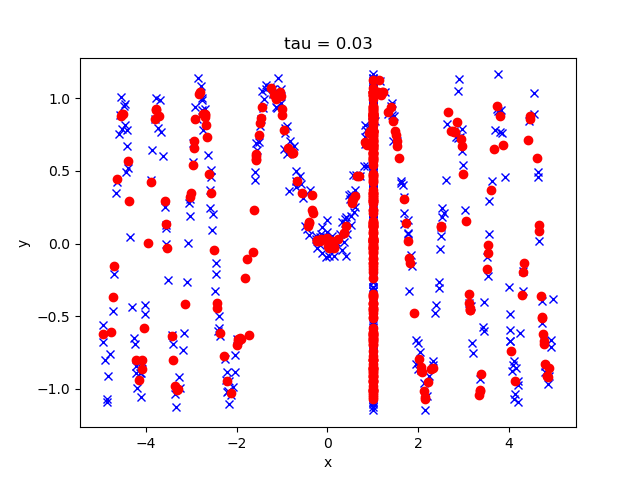
\includegraphics[width=1\textwidth]{images/p05c_tau_0.03.png}
  \caption{$\tau=0.03$}
  \label{fig:enter-label}
\end{figure}

\begin{figure}
  \centering
  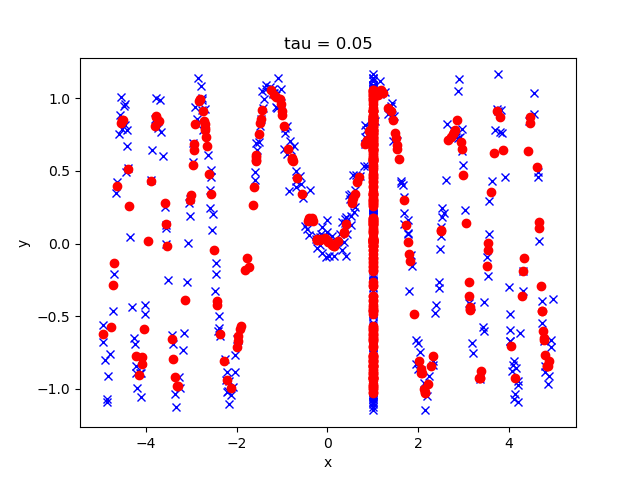
\includegraphics[width=1\textwidth]{images/p05c_tau_0.05.png}
  \caption{$\tau=0.05$}
  \label{fig:enter-label}
\end{figure}

\begin{figure}
  \centering
  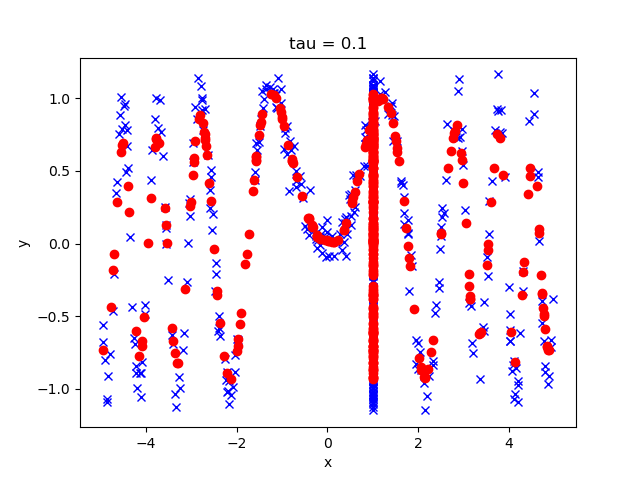
\includegraphics[width=1\textwidth]{images/p05c_tau_0.1.png}
  \caption{$\tau=0.1$}
  \label{fig:enter-label}
\end{figure}

\begin{figure}[h]
  \centering
  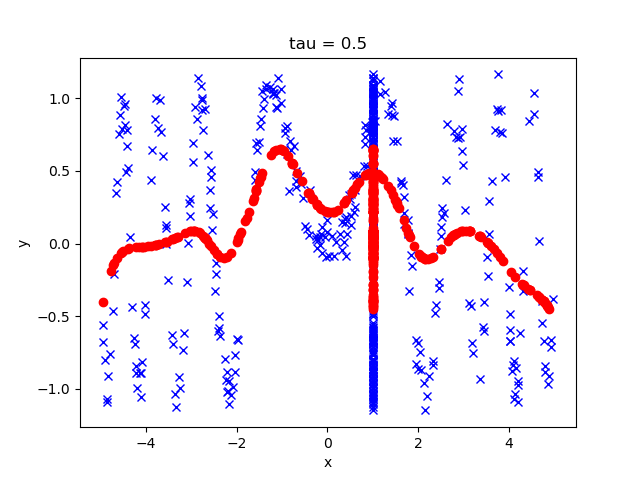
\includegraphics[width=1\textwidth]{images/p05c_tau_0.5.png}
  \caption{$\tau=0.5$}
  \label{fig:enter-label}
\end{figure}

\begin{figure}[h]
  \centering
  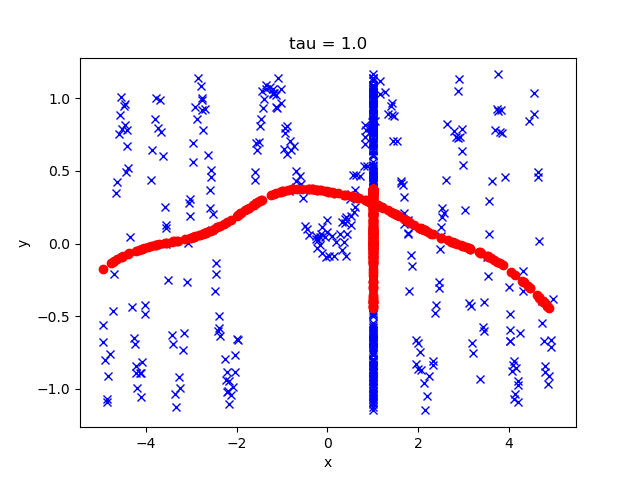
\includegraphics[width=1\textwidth]{images/p05c_tau_1.0.png}
  \caption{$\tau=1.0$}
  \label{fig:enter-label}
\end{figure}

\begin{figure}[h]
  \centering
  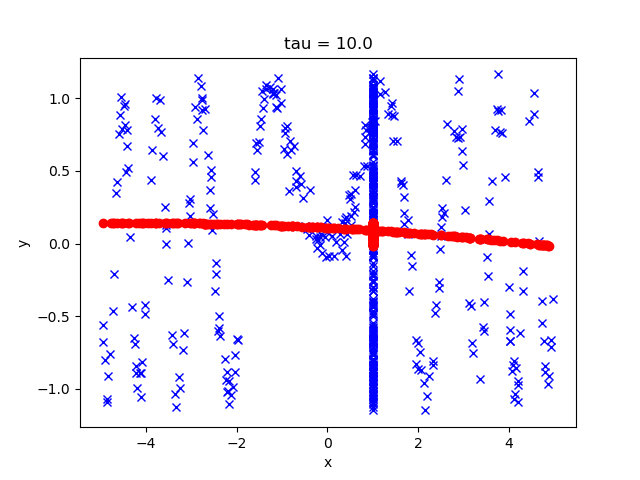
\includegraphics[width=1\textwidth]{images/p05c_tau_10.0.png}
  \caption{$\tau=10.0$}
  \label{fig:enter-label}
\end{figure}

$\tau=0.05$ got the lowest MSE on the validation set(0.012), and 0.017 on the test set

\end{document}

